\documentclass[a4paper,twoside,11pt]{article}
\usepackage{a4wide,graphicx,fancyhdr,amsmath,amssymb,amsthm,ifthen,path}
\usepackage[ruled, noline, algo2e, noend]{algorithm2e}
\usepackage{hyperref}
\usepackage{url}
\usepackage{color}
\usepackage{todonotes}
\usepackage{parskip}
\usepackage{subcaption}
\usepackage{etoolbox, array, dcolumn}
\usepackage{enumitem}   

\urlstyle{rm}

\setlength\headheight{20pt}
\addtolength\topmargin{-10pt}
\addtolength\footskip{20pt}

\fancypagestyle{plain}{%
	\fancyhf{}
	\fancyfoot[LO,RE]{\sffamily\bfseries 2IV35~--~Visualization}
	\fancyfoot[RO,LE]{\sffamily\bfseries\thepage}
	\renewcommand{\headrulewidth}{0pt}
	\renewcommand{\footrulewidth}{0pt}
}

\pagestyle{fancy}{
\fancyhf{}
\fancyhead[LE]{\sffamily\bfseries Joris Reijrink and Chris Hoedemakers}
\fancyhead[RO]{\sffamily\bfseries Interactive Visualization}
\fancyfoot[LO,RE]{\sffamily\bfseries 2IV35~--~Visualization}
\fancyfoot[RO,LE]{\sffamily\bfseries\thepage}
\renewcommand{\headrulewidth}{1pt}
\renewcommand{\footrulewidth}{0pt}
}

\title{\sffamily\bfseries
\fontsize{22pt}{1pt} Assignment 3 \\[1ex]
\large Interactive Visualization \bigskip}

\author{
	Joris Reijrink \\
	Student number: 0847198 \\
	\texttt{j.reijrink@student.tue.nl}
	\and
	Chris Hoedemakers \\
	Student number: 0661115 \\
	\texttt{c.g.j.j.hoedemakers@student.tue.nl}
}

\date{\today}

\newcounter{cs}

\newcommand{\code}[1]{
	\refstepcounter{cs}
	\begin{center}
	\hspace*{-2.2cm}
	\begin{minipage}{1.103\textwidth}
		\begin{minipage}{0.1\textwidth}%
			\raggedleft
			\footnotesize{\texttt{CS \thecs}}\hspace*{0.3cm}
		\end{minipage}
		\begin{minipage}{0.88\textwidth}%
			\colorbox{gray!20}{
				\begin{minipage}{\textwidth}%
				\fontsize{8pt}{8pt}\texttt{#1}
				\end{minipage}
			}
		\end{minipage}
	\end{minipage}
	\end{center}
	\vspace*{0.3cm}
}
\newcommand{\tab}{\hspace*{0.6cm}}

\newcolumntype{d}[1]{D{.}{.}{#1}}


\begin{document}

\maketitle
\setcounter{page}{1}

\setlength{\parindent}{0cm}
\setlength{\parskip}{0.3cm}

\section{Introduction}
In this report we ...
\section{Data Set}\label{sec:data}




\section{Tasks}\label{sec:tasks}

In this section we define the tasks that we would like to perform. That is, we describe what information we would like to retrieve from the given data set. Before we define these tasks we provide a framework (or design space) for formulating specific tasks.

\subsection{Framework for Defining Tasks}
In order to formulate a nice and clear visualization task, we define a framework for doing this as described in \cite{schulz2013design}. Here we distinguish between five different dimensions for each task, namely the \textit{goal} (why is the task pursued), \textit{means} (how is the task carried out), \textit{characteristics}(what does the task seek), \textit{target} (on which part of the data is the task carried out) and \textit{cardinality} (on how many instances is the task carried out). We shortly explain these five aspects in some more detail.

For the goal of the task we distinguish between three different types of analyses. We can have an exploratory analysis (or undirected search) that aims at deriving an hypothesis from an unknown data set, a confirmatory analysis (directed search)

\todo{!}...

\subsection{Chosen Tasks}
With this common framework for formulating visualization tasks defined, we move on to defining the actual tasks we want to perform on our data set about the Dutch municipalities. We mainly distinguish between two different tasks, of which the first one will be divided into two subtasks.

\subsubsection{Task 1}\label{sec:task1}
The first task that we define aims at discovering interesting properties of the given data set, as well as confirming expected properties. This means that this task is actually rather broad, and numerous specific questions can be formulated from it. However, we will define two basic (sub)tasks for analyzing the entire data set, namely\textit{a)'analyze the relations between the different attributes'} in the set, and \textit{b) 'compare the attribute values of the different municipalities with each other'}. The subset of attributes on which we will perform both of these tasks will be the same. This subset will consist of the attributes \texttt{OAD}, \texttt{STED}, \texttt{AANT\_INW}, \texttt{BEV\_DICHTH}, \texttt{AANTAL\_HH}, \texttt{P\_EENP\_HH}, and \texttt{OPP\_TOT}. For convenience we will call this set of attributes $S_{attr}$.

When formally defining task 1a, we observe that we adopt an \textit{exploratory} approach, as we aim at \textit{searching} interesting \textit{relations} between different data set attributes. From this we can (partly) derive the first three dimensions for our 5-tuple task description. The forth dimensions, the target has also been specified already, namely $s_{attr}$. This leaves us with the cardinality. Because we want to discover general relations, we want to look at all data instances (municipalities). However, some relations between attributes may be very obvious. We will therefore also be looking for \textit{confirmation} of these obvious relations, and want to detect possible abnormalities or inconsistencies in them, such as \textit{outliers}. The resulting formal task description then looks like this:

(exploratory|confirmatory, relation-seeking, relations|outliers, $S_{attr}$, all)

For task 1b we can define a somewhat similar task. The main difference is now that we will not be looking at the relations between the different data attributes, but are \textit{comparing} the data values of the different data objects. In this way we again hope to find interesting characteristics such as \textit{outliers} or \textit{clusters}. As with task 1a, we again take $S_{attr}$ as our target and all instances as cardinality.

(exploratory|confirmatory, comparison, outliers|clusters, $S_{attr}$, all)

Specific questions that we could pose for the first of these two subtasks is for instance 'is there a positive relation between the attributes \texttt{AANT\_INW} and \texttt{BEV\_DICHTH}?'. If we think about this for a minute in advance, we may expect that this will indeed be the case. Hence this would be a typical question where we try to confirm our hypothesis, and look for data objects that do not adhere to this. A much more general and exploratory question would be 'which attributes have a typical positive or negative relation with each other?'. Again we may define some expected relations, such as a negative relation between \texttt{OAD} and \texttt{STED}. However, this question really aims for elaborate (though high level) analysis of the data.

For task 1b we can also define a question of which we can already guess the answer. We could for instance confirm that the four largest cities in the Netherlands score the highest on the \texttt{AANT\_INW} attribute. Furthermore we may expect these values to be rather significantly larger than those of the other municipalities. Finally we may again pose a general, exploratory question in the form of 'how are the attribute values of the municipalities distributed for a certain attribute, and can we explain this distribution?'.




\subsubsection{Task 2}\label{sec:task2}
In this task we search for confirmation to a specific question.
This question is formulated based on a hypothesis on which we seek validation.
Once the question is answered it can be used to support the hypotheses.\\
\\
The specific question we want an answer to is whether there are municipalities in the Netherlands that suffer from a high degree of an aging population ('vergrijzing' in Dutch).
This question is based on the hypothesis that the Netherlands is suffering of a high degree aging population.\\
The degree of aging population is based on the inhabitants that are older than 65 years, and the working inhabitants.
The working inhabitants are defined as the age group from 20 till 65, this is not the actual group of working inhabitants but it is a good representation.
\\
The specific question can be described as a formal task description:\\
(\textit{confirmatory, searching localization, attr($P\_00\_14\_JR$, $P\_15\_19\_JR$, $P\_20\_24\_JR$, $P\_25\_44\_JR$, $P\_45\_64\_JR$, $P\_65\_EO\_JR$), all})\\
\\
The formal task describes that the user is searching confirmation among all available 65+-percentage attribute values and the 20- till 64-percentage attribute values, this last attribute is created with a combination of different percentage attributes.
The task is confirmatory, so the user knows what he is looking for and seeking confirmation to what he wants to prove.
The user is looking at low-level data characteristics (localization), this means no complex patterns in the data but simply searching for the high valued attribute values in the data objects (municipalities). 
\section{Techniques}

\subsection{techniques for task 1}
\todo{foreseen pros and cons}

Techniques that can be chosen for this broad exploration of the data include a Parallel Coordinate Plot (PCP) and Scatterplot Matrix (SM). This is because these two techniques enable us to show a lot of different attributes in one large overview. An advantage of the PCP over the SM is however that the PCP tends to take up less space. Also the axes of the SM tend to become very small when numerous attributes are used. This makes it hard to distinguish between single data objects when analyzing the data. When data objects can be be categorized, this problem can be partly overcome by specifying each category with a certain color. However, for our municipalities data set this categorization is not really possible. An imaginable solution for this would be an interactive SM where the user can zoom in on one of the scatterplots. Unfortunately D3 \cite{D3} does not provide such an example, and implementing it ourselves was considered to consume too much time. For these reasons, it was chosen do use a PCP.

con: outliers rack up the scaling -> solution: scale the axes to selection


\subsection{techniques for task 2}
- bar chart
 - absolute vergelijken
 - niet de relaties tot elkaar mbt percentages
 
- normalized bar chart
 - eenvoudig vergelijken
 
- choropleth map
 - eenvoudig vergelijken
 - moeilijk kleuren onderscheiden
 
- scatter plot

- sunburst
 - teveel gemeenten
 - geen hierarchische data

- pyramid
 - alleen top 10?
 
 
\todo{optional techniques}
\todo{pro cons}
\todo{argueing for chosen technique}


\section{Observations}

\subsection{Observations Task 1}
\todo{what information could be retrieved from the implemented technique?}
\todo{was the task accomplished?}
\todo{pros, cons, improvements}

task 1a
- taking some general attributes such as those in $S_{attr}$ mainly show rather obvious relations:
    > \texttt{AANTAL\_INW} == \texttt{AANTAL\_HH}
    > \texttt{OPP\_TOT} inverse \texttt{BEV\_DICHTH}
    > \texttt{STED} inverse \texttt{OAD}
- quite some attributes with a few outliers that mess up the scale of the axis
\texttt{OPP\_TOT}, \texttt{OAD}, \texttt{AANTAL\_INW}, \texttt{AANTAL\_HH}
    this makes it harder to detect relations between the attributes of the more general municipalities, because they lie very close to each other on the axis.

Let us now the questions we posed in the section Tasks,
- answers to questions: \texttt{AANT\_INW} <-> \texttt{BEV\_DICHTH}: Súdwest-Fryslân, Lelystad, Haarlemmermeer, Apeldoorn, Ede, Emmen do not adhere


task 1b
- again because the scaling, it also becomes harder to compare municipalities
\texttt{OPP\_TOT}, \texttt{OAD}, \texttt{AANTAL\_HH},
-> con: outliers rack up the scaling -> solution: scale the axes to selection
- student cities have highest percentage of single households (\texttt{P\_EENP\_HH})
- municipalicites with low \texttt{STED} value fluctuate more on the other attributes

\begin{figure}[h!]
    \centering
    \captionsetup{justification=centering,margin=2cm}
    \begin{subfigure}[t]{0.48\textwidth}
        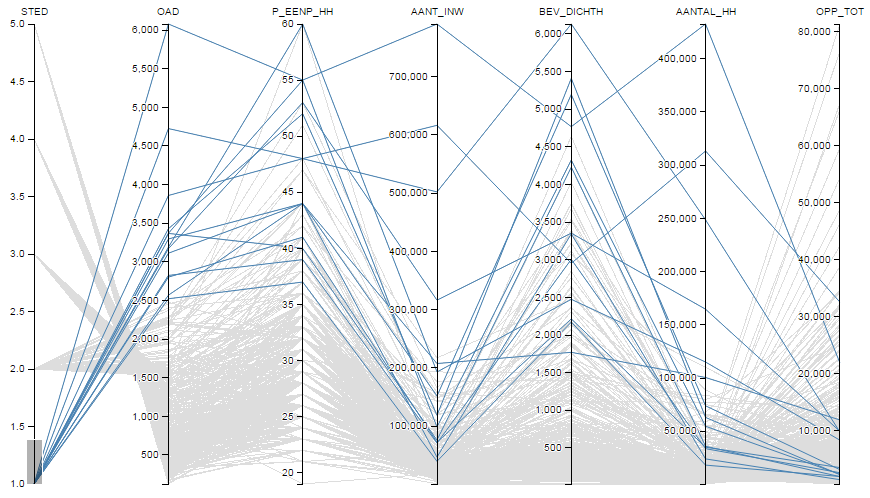
\includegraphics[width=\textwidth]{img/pcp_STED1.png}
        \caption{ }
    \end{subfigure}
    \begin{subfigure}[t]{0.48\textwidth}
        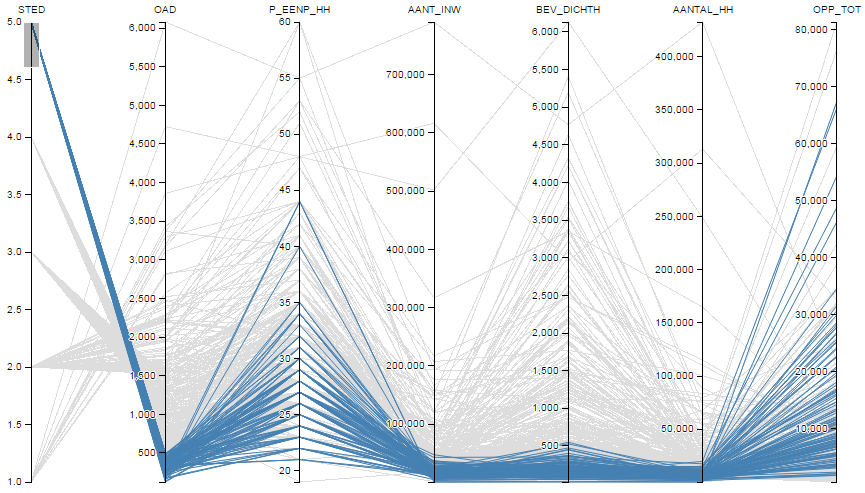
\includegraphics[width=\textwidth]{img/pcp_STED5.png}
        \caption{ }
    \end{subfigure}
    \label{fig:pcp_sted}
    \caption{Parallel Coordinate Plots highlighting the municipalities with a \texttt{STED} value of 1 (a), and a \texttt{STED} value of 5 (b)}
\end{figure}

\subsection{Observations Task 2}
\todo{what information could be retrieved from the implemented technique?}
\todo{was the task accomplished?}
\todo{pros, cons, improvements}



\bibliographystyle{plain}
\bibliography{bibliography}

\appendix

\section{Appendix: Dataset}\label{app:appData}
The data attributes are described using the following format:\\
\textbf{attribute name} [type]: description\\% [range]\\
\\
\textbf{\large 1. chefmozaccepts.csv}\\
\\
\textbf{placeID} [number]: unique identifier of the restaurant\\
\textbf{Rpayment} [text]: describes the payment methods the restaurants accepts\\
\\
\textbf{\large 2. chefmozcuisine.csv}\\
\\
\textbf{placeID} [number]: unique identifier of the restaurant\\
\textbf{Rcuisine} [text]: describes the present cuisines of the restaurants\\
\\
\textbf{\large 3. chefmozhours4.csv}\\
\\
\textbf{placeID} [number]: unique identifier of the restaurant\\
\textbf{hours} [text]: opening hours of the restaurant in 00:00-23:59 format\\
\textbf{days} [text]: days in the week the restaurant is open, days are separated with semicolon\\
\\
\textbf{\large 4. chefmozparking.csv}\\
\\
\textbf{placeID} [number]: unique identifier of the restaurant\\
\textbf{parking} [text]: describes the parking possibilities of the restaurant\\
\\
\textbf{\large 5. geoplaces2.csv}\\
\\
\textbf{placeID} [number]: unique identifier of the restaurant\\
\textbf{latitude} [number]: latitude of the restaurant location\\
\textbf{longitude} [number]: longitude of the restaurant location\\
\textbf{the\_geom\_meter} [number]: geospatial name of the restaurant\\
\textbf{name} [text]: restaurant name\\
\textbf{address} [text]: restaurant address\\
\textbf{city} [text]: city where the restaurant is located\\
\textbf{state} [text]: state where the restaurant is located\\
\textbf{country} [text]: country where the restaurant is located\\
\textbf{fax} [text]: fax number of the restaurant\\
\textbf{zip} [text]: zip code where the restaurant is located\\
\textbf{alcohol} [text]: describes if the restaurant serves alcohol\\
\textbf{smoking\_area} [text]: described if the restaurant permits smoking inside\\
\textbf{dress\_code} [text]: restaurants type of dress code\\
\textbf{accessibility} [text]: accessibility for disabled\\
\textbf{price} [text]: overall pricing of the restaurant, this can be low, medium or high\\
\textbf{url} [text]: restaurant website url\\
\textbf{Rambience} [text]: ambience of the restaurant, this can be familiar or quiet\\
\textbf{franchise} [boolean]: is the restaurant part of a franchise\\
\textbf{area} [text]: area of the restaurant\\
\textbf{other\_services} [text]: other services provided by the restaurant\\
\\
\textbf{\large 6. usercuisine.csv}\\
\\
\textbf{userID} [number]: unique identifier of the consumer\\
\textbf{Rcuisine} [text]: the preferred cuisine of the consumer, a user can have multiple\\
\\
\textbf{\large 7. userpayment.csv}\\
\\
\textbf{userID} [number]: unique identifier of the consumer\\
\textbf{Upayment} [text]: payment methods the consumer has used in restaurants\\
\\



\textbf{\large 8. userprofile.csv}\\
\\
\textbf{userID} [number]: unique identifier of the consumer\\
\textbf{latitude} [number]: latitude of the consumer's home\\
\textbf{longitude} [number]: longitude of the consumer's home\\
\textbf{the\_geom\_meter} [number]: geospatial name of the consumer's home location\\
\textbf{smoker} [boolean]: is the consumer a smoker\\
\textbf{drink\_level} [text]: drinking level of the consumer\\
\textbf{dress\_preference} [text]: dress code preference of the consumer\\
\textbf{ambience} [text]: ambience preference of the consumer\\
\textbf{transport} [text]: transportation preference of the consumer\\
\textbf{marital\_status} [text]: marital status of the consumer\\
\textbf{hijos} [text]: children status of the consumer\\
\textbf{birth\_year} [text]: birth year of the consumer\\
\textbf{interest} [text]: interests of the consumer\\
\textbf{personality} [text]: personality of the consumer\\
\textbf{religion} [text]: religion of the consumer\\
\textbf{activity} [text]: work status, this can be student, professional, unemployed or working-class\\
\textbf{color} [text]: favorite color of the consumer\\
\textbf{weight} [number]: weight of the consumer\\
\textbf{budget} [text]: food budget of the consumer, this can be low, medium or high\\
\textbf{height} [number]: height of the consumer\\
\\
\textbf{\large 9. rating\_final.csv}\\
\\
\textbf{userID} [number]: unique identifier of the consumer\\
\textbf{placeID} [number]: unique identifier of the restaurant\\
\textbf{rating} [number]: the overall rating of the consumer at a specific restaurant\\
\textbf{food\_rating} [number]: the food rating of the consumer at a specific restaurant\\
\textbf{service\_rating} [number]: the service rating of the consumer at a specific restaurant

\section{Appendix: Work breakdown}\label{app:appB}


\begin{center}
  \begin{tabular}{| c | c |}
    \hline
    Joris & Chris \\ \hline\hline
    \multicolumn{2}{|c|}{Report} \\ \hline\hline
    data set &  introduction\\ \hline
    appendix A &  tasks\\ \hline
    implementation &  techniques\\ \hline
    improvements & observations \\ \hline\hline
     &  \\ \hline\hline
    \multicolumn{2}{|c|}{Implementation} \\ \hline\hline
    geographic map pane & parallel coordinate plot pane \\ \hline
    average rating pane &  \\ \hline
    restaurant / consumer information pane &  \\ \hline
     &  \\ \hline
  \end{tabular}
\end{center}





\end{document}
